\documentclass[journal,12pt,twocolumn]{IEEEtran}
\usepackage[shortlabels]{enumitem}
\usepackage{setspace}
\usepackage{gensymb}
\singlespacing
\usepackage[cmex10]{amsmath}
\usepackage{graphicx}

\usepackage{float}
\usepackage{amsthm}

\usepackage{mathrsfs}
\usepackage{txfonts}
\usepackage{stfloats}
\usepackage{bm}
\usepackage{cite}
\usepackage{cases}
\usepackage{subfig}

\usepackage{longtable}
\usepackage{multirow}

\usepackage{enumitem}
\usepackage{mathtools}
\usepackage{steinmetz}
\usepackage{tikz}
\usepackage{circuitikz}
\usepackage{verbatim}
\usepackage{tfrupee}
\usepackage[breaklinks=true]{hyperref}
\usepackage{graphicx}
\usepackage{tkz-euclide}

\usetikzlibrary{calc,math}
\usepackage{listings}
    \usepackage{color}                                            %%
    \usepackage{array}                                            %%
    \usepackage{longtable}                                        %%
    \usepackage{calc}                                             %%
    \usepackage{multirow}                                         %%
    \usepackage{hhline}                                           %%
    \usepackage{ifthen}                                           %%
    \usepackage{lscape}     
\usepackage{multicol}
\usepackage{chngcntr}

\DeclareMathOperator*{\Res}{Res}

\renewcommand\thesection{\arabic{section}}
\renewcommand\thesubsection{\thesection.\arabic{subsection}}
\renewcommand\thesubsubsection{\thesubsection.\arabic{subsubsection}}

\renewcommand\thesectiondis{\arabic{section}}
\renewcommand\thesubsectiondis{\thesectiondis.\arabic{subsection}}
\renewcommand\thesubsubsectiondis{\thesubsectiondis.\arabic{subsubsection}}


\hyphenation{op-tical net-works semi-conduc-tor}
\def\inputGnumericTable{}                                 %%

\lstset{
%language=C,
frame=single, 
breaklines=true,
columns=fullflexible
}
\begin{document}

\newcommand{\BEQA}{\begin{eqnarray}}
\newcommand{\EEQA}{\end{eqnarray}}
\newcommand{\define}{\stackrel{\triangle}{=}}
\bibliographystyle{IEEEtran}
\raggedbottom
\setlength{\parindent}{0pt}
\providecommand{\mbf}{\mathbf}
\providecommand{\pr}[1]{\ensuremath{\Pr\left(#1\right)}}
\providecommand{\qfunc}[1]{\ensuremath{Q\left(#1\right)}}
\providecommand{\sbrak}[1]{\ensuremath{{}\left[#1\right]}}
\providecommand{\lsbrak}[1]{\ensuremath{{}\left[#1\right.}}
\providecommand{\rsbrak}[1]{\ensuremath{{}\left.#1\right]}}
\providecommand{\brak}[1]{\ensuremath{\left(#1\right)}}
\providecommand{\lbrak}[1]{\ensuremath{\left(#1\right.}}
\providecommand{\rbrak}[1]{\ensuremath{\left.#1\right)}}
\providecommand{\cbrak}[1]{\ensuremath{\left\{#1\right\}}}
\providecommand{\lcbrak}[1]{\ensuremath{\left\{#1\right.}}
\providecommand{\rcbrak}[1]{\ensuremath{\left.#1\right\}}}
\theoremstyle{remark}
\newtheorem{rem}{Remark}
\newcommand{\sgn}{\mathop{\mathrm{sgn}}}
\providecommand{\abs}[1]{\vert#1\vert}
\providecommand{\res}[1]{\Res\displaylimits_{#1}} 
\providecommand{\norm}[1]{\lVert#1\rVert}
%\providecommand{\norm}[1]{\lVert#1\rVert}
\providecommand{\mtx}[1]{\mathbf{#1}}
\providecommand{\mean}[1]{E[ #1 ]}
\providecommand{\fourier}{\overset{\mathcal{F}}{ \rightleftharpoons}}
%\providecommand{\hilbert}{\overset{\mathcal{H}}{ \rightleftharpoons}}
\providecommand{\system}{\overset{\mathcal{H}}{ \longleftrightarrow}}
	%\newcommand{\solution}[2]{\textbf{Solution:}{#1}}
\newcommand{\solution}{\noindent \textbf{Solution: }}
\newcommand{\cosec}{\,\text{cosec}\,}
\providecommand{\dec}[2]{\ensuremath{\overset{#1}{\underset{#2}{\gtrless}}}}
\newcommand{\myvec}[1]{\ensuremath{\begin{pmatrix}#1\end{pmatrix}}}
\newcommand{\mydet}[1]{\ensuremath{\begin{vmatrix}#1\end{vmatrix}}}
\numberwithin{equation}{subsection}
\makeatletter
\@addtoreset{figure}{problem}
\makeatother
\let\StandardTheFigure\thefigure
\let\vec\mathbf
\renewcommand{\thefigure}{\theproblem}
\def\putbox#1#2#3{\makebox[0in][l]{\makebox[#1][l]{}\raisebox{\baselineskip}[0in][0in]{\raisebox{#2}[0in][0in]{#3}}}}
     \def\rightbox#1{\makebox[0in][r]{#1}}
     \def\centbox#1{\makebox[0in]{#1}}
     \def\topbox#1{\raisebox{-\baselineskip}[0in][0in]{#1}}
     \def\midbox#1{\raisebox{-0.5\baselineskip}[0in][0in]{#1}}
\vspace{3cm}
\title{Assignment 2}
\author{CS20BTECH11028}
\maketitle
\newpage
\bigskip
\renewcommand{\thefigure}{\theenumi}
\renewcommand{\thetable}{\theenumi}
%
and latex-tikz codes from 
%
\begin{lstlisting}
    https://github.com/Harsha24112002/AI1103/tree/main/Assignment-2
\end{lstlisting}
\section{Problem GATE EC 56}
Let $X$ and $Y$ be jointly distributed random variables such that the conditional distribution of $Y$, given $X$ =$x$, is uniform on the interval $(x-1,x+1)$. Suppose $E(X)=1$ and $Var(X)=\frac{5}{3}$.
\\
 The mean of the random variable $Y$ is 
\\
\begin{enumerate}[(A)]
\begin{multicols}{2}
\setlength\itemsep{1em}

\item $ \frac{1}{2}$\\
\item $1$\\
\item $ \frac{3}{2}$\\
\item $2$

\end{multicols}
\end{enumerate}
\section{Solution GATE EC 56}
We know that,
\begin{equation}
    \Pr{(Y=y|X=x)}=\frac{f(x,y)}{f_1(x)} \label{eq:2.0.1}
\end{equation}
where $f(x,y)=\Pr(X=x,Y=y)$.,$f_1(x)$ is the marginal probability for X=x.\\
Given that $\Pr{(Y|X=x)}$ is uniform over the interval (x-1,x+1).
\begin{align}
    \Rightarrow \Pr{(Y=y|X=x)} &= \frac{1}{(x+1)-(x-1)}\\
    &=\frac{1}{2}
\end{align}
\begin{equation}
    \Rightarrow \Pr{(Y=y|X=x)}=
    \begin{cases}
    \frac{1}{2} & y \in \brak{x-1,x+1}\\
    0 & \text{otherwise}
    \end{cases}\label{eq:2.0.4}
\end{equation}
\begin{figure}[H]
    \centering
    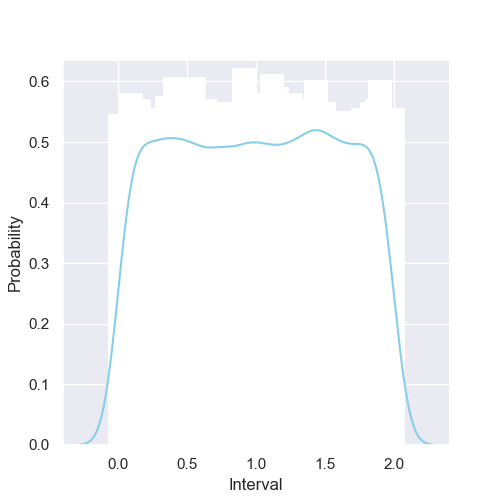
\includegraphics[scale=0.6]{assignment 2.png}
    \caption{Distribution of $\Pr{(Y=y|X=1)}$}
\end{figure}
Given $E(X)=1$
\begin{equation}
    \Rightarrow \int_{-\infty}^{\infty}x f_{1}(x)dx=1 \label{eq:2.0.5}
\end{equation}
Now consider $E(Y)$,
\begin{equation}
    E(Y)=\int_{-\infty}^{\infty}yf_{1}(y)dy
\end{equation}
As $f_{1}(y)$ is a marginal probability of Y=y we can write as,
\begin{equation}
    E(Y)=\int_{-\infty}^{\infty}\int_{-\infty}^{\infty}y f(x,y)dx dy
\end{equation}
From \ref{eq:2.0.1} we can write ,
\begin{align}
    E(Y)&=\int_{-\infty}^{\infty}\int_{-\infty}^{\infty}y \Pr{(Y=y|X=x)} f_{1}(x) dx dy\\
    &=\int_{-\infty}^{\infty}\brak{\int_{-\infty}^{\infty}y \Pr{(Y=y|X=x)}dy} f_{1}(x) dx
\end{align}
From \ref{eq:2.0.4} we can simplify as,
\begin{align}
    E(Y)&=\int_{-\infty}^{\infty}\brak{\int_{(x-1)}^{(x+1)}y \Pr{(Y=y|X=x)}dy} f_{1}(x) dx\\
    &=\int_{-\infty}^{\infty}\brak{\int_{(x-1)}^{(x+1)}y \brak{\frac{1}{2}} dy} f_{1}(x) dx\\
    &=\int_{-\infty}^{\infty} \brak{\frac{1}{2}} \brak{\frac{(x+1)^2-(x-1)^2}{2}}  f_{1}(x) dx\\
    &= \int_{-\infty}^{\infty}x f_{1}(x)dx\\
    &=E(X)
\end{align}
Hence from \ref{eq:2.0.5} it can be seen that 
\begin{equation}
    E(Y)=1
\end{equation}
\textbf{$\therefore$ Option B is true}

%In the question there was no information about the distribution of X and distribution Y, only distribution of Y given X=x is given.So i did not write a code for simulation sir%

\end{document}
